\documentclass{epflreport}%
\usepackage[T1]{fontenc}%
\usepackage[utf8]{inputenc}%
\usepackage{lmodern}%
\usepackage{textcomp}%
\usepackage{lastpage}%
\usepackage{graphicx}%
\usepackage{longtable}%
%
%
%
\begin{document}%
\normalsize%
\frontmatter%
\title{Gothenburg patient study}%
\subtitle{rifampicin (key results)}%
\author{miblab.org}%
\subject{D2.13 {-} Internal report}%
\affiliation{https://miblab.org}%
\coverimage{cover.jpg}%
\definecolor{title}{HTML}{FF0000}%
\makecover%
\begin{titlepage}%
\begin{center}%
\makeatletter%
\largetitlestyle\fontsize{45}{45}\selectfont\@title%
\makeatother%
\linebreak%
\makeatletter%
\ifdefvoid{\@subtitle}{}{\bigskip\titlestyle\fontsize{20}{20}\selectfont\@subtitle}%
\makeatother%
\linebreak%
\bigskip%
\bigskip%
by%
\linebreak%
\bigskip%
\bigskip%
\makeatletter%
\largetitlestyle\fontsize{25}{25}\selectfont\@author%
\makeatother%
\vfill%
\large%
\begin{tabular}{ll}%
\hline%
Report compiled by: &Steven Sourbron\\%
Institute: &University of Sheffield\\%
Department: &Section of Medical Imaging and Technologies\\%
Email: &s.sourbron@sheffield.ac.uk\\%
Date: &\today\\%
\hline%
\end{tabular}%


\begin{figure}[b!]%
\centering%
\centering%

\includegraphics[width=2in]{C:/Users/md1spsx/Documents/GitHub/tristan-human-modelling/build/rifampicin_clinical/report (summary)_source/layout/tristan-logo.jpg}%
\end{figure}

%
\end{center}%
\end{titlepage}%
\newpage%
\tableofcontents%
\mainmatter%
\clearpage%
\chapter{Key results}%
\section{Data summary}%
\label{sec:Datasummary}%

%


\begin{figure}[h!]%
\centering%
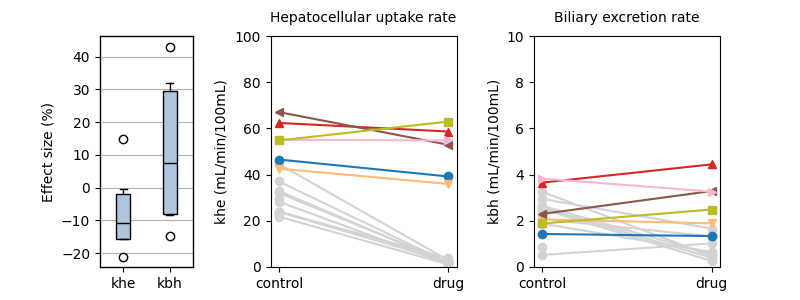
\includegraphics[width=7in]{C:/Users/md1spsx/Documents/GitHub/tristan-human-modelling/build/rifampicin_clinical/results (two scans)/Figures/_effect_plot.png}%
\caption{Effect size (\%) on hepatocellular uptake (k\_he, left) and biliary excretion (k\_bh, right) of gadoxetate. The boxplot shows median, interquartile range and 95 percent range. The line plots show individual values for hepatocellular uptake (k\_he, middle) and biliary excretion (k\_bh, right) of gadoxetate of the control (left of plot) and treatment (right of plot). Grey lines are healthy controls with rifampicin injection.}%
\end{figure}

%
\begin{longtable}{rcccccccc}%
\hline%
parameter&count&mean&std&min&25\%&50\%&75\%&max\\%
\hline%
khe effect size (\%)&3.0&{-}25.2&56.3&{-}83.6&{-}52.2&{-}20.8&4.0&28.7\\%
khe control (mL/min/100cm3)&3.0&9.62&6.17&2.53&7.57&12.6&13.17&13.74\\%
khe drug (mL/min/100cm3)&3.0&5.4&4.78&2.07&2.67&3.26&7.07&10.88\\%
kbh effect size (\%)&3.0&89.1&45.4&48.7&64.6&80.5&109.4&138.3\\%
kbh control (mL/min/100cm3)&3.0&2.37&1.73&0.51&1.58&2.66&3.29&3.93\\%
kbh drug (mL/min/100cm3)&3.0&4.36&3.0&0.92&3.38&5.84&6.09&6.34\\%
\hline%
\caption{Effect size and absolute values of hepatocellular uptake (k\_he) and biliary excretion (k\_bh) of gadoxetate} \\%
\end{longtable}%
\clearpage%
\section{Liver biomarkers}%
\label{sec:Liverbiomarkers}%

%
\begin{longtable}{rccc}%
\hline%
Biomarker&p{-}value&Bayes Factor&Odds Ratio\\%
\hline%
AUC for Cl (0{-}35min)&0.25099&0.92&4.79\\%
AUC for Cl (0{-}inf)&0.3815&0.7&3.97\\%
Biliary excretion rate&0.16853&1.19&0.23\\%
Biliary tissue excretion rate&0.21172&1.03&0.27\\%
Extracellular dispersion&0.09444&1.73&4.09\\%
Extracellular mean transit time&0.99189&0.47&0.99\\%
Final biliary excretion rate&0.2935&0.83&0.2\\%
Final hepatocellular uptake rate&0.58834&0.55&2.52\\%
Hematocrit&&&\\%
Hepatocellular mean transit time&0.1663&1.2&1.89\\%
Hepatocellular tissue uptake rate&0.9649&0.47&1.07\\%
Hepatocellular uptake rate&0.33144&0.77&4.0\\%
Initial biliary excretion rate&0.96252&0.47&0.9\\%
Initial hepatocellular uptake rate&0.24237&0.94&5.81\\%
Liver T1{-}MOLLI at 45min&0.98716&0.47&1.01\\%
Liver T1{-}MOLLI at baseline&0.07944&1.93&3.61\\%
Liver T1{-}MOLLI at scan 2&0.54424&0.57&0.74\\%
Liver blood clearance&0.35827&0.73&2.55\\%
Liver extracellular volume fraction&0.13135&1.4&10.13\\%
RE for R1l at 20min&0.22432&0.99&8.14\\%
RE for Sl at 20min&0.2206&1.0&7.44\\%
\hline%
\caption{Results of a pairwise comparison testing for differences in liver biomarkers between control and treatment. The results are ranked by their p-value, with most significant differences at the top of the list.} \\%
\end{longtable}%
\begin{longtable}{rcccc}%
\hline%
Biomarker&Units&control&drug&change (\%)\\%
\hline%
AUC for Cl (0{-}35min)&mM*sec&54.3 (33.0) &34.8 (15.0) &{-}25.7 (44.0) \\%
AUC for Cl (0{-}inf)&mM*sec&289.0 (420.0) &86.7 (67.0) &{-}36.7 (64.0) \\%
Biliary excretion rate&mL/min/100cm3&2.37 (2.0) &4.36 (3.4) &89.1 (51.0) \\%
Biliary tissue excretion rate&mL/min/100cm3&3.23 (2.4) &5.52 (4.4) &64.8 (51.0) \\%
Extracellular dispersion&\%&84.6 (5.6) &79.7 (8.3) &{-}5.85 (3.9) \\%
Extracellular mean transit time&sec&52.4 (9.4) &52.5 (7.4) &1.02 (15.0) \\%
Final biliary excretion rate&mL/min/100cm3&3.38 (3.7) &5.46 (0.78) &593.0 (1100.0) \\%
Final hepatocellular uptake rate&mL/min/100cm3&11.1 (9.4) &7.04 (8.8) &{-}1.57 (90.0) \\%
Hematocrit&\%&45.0 (0.0) &45.0 (0.0) &0.0 (0.0) \\%
Hepatocellular mean transit time&min&55.3 (64.0) &37.7 (48.0) &{-}36.5 (17.0) \\%
Hepatocellular tissue uptake rate&mL/min/100cm3&28.8 (16.0) &28.1 (26.0) &17.6 (97.0) \\%
Hepatocellular uptake rate&mL/min/100cm3&9.62 (7.0) &5.4 (5.4) &{-}25.2 (64.0) \\%
Initial biliary excretion rate&mL/min/100cm3&4.3 (2.6) &4.47 (3.9) &74.5 (220.0) \\%
Initial hepatocellular uptake rate&mL/min/100cm3&8.1 (6.9) &3.77 (2.0) &{-}39.5 (43.0) \\%
Liver T1{-}MOLLI at 45min&sec&0.793 (0.14) &0.793 (0.13) &0.33 (10.0) \\%
Liver T1{-}MOLLI at baseline&sec&0.983 (0.12) &0.916 (0.089) &{-}6.57 (3.5) \\%
Liver T1{-}MOLLI at scan 2&sec&0.807 (0.16) &0.827 (0.11) &3.25 (8.1) \\%
Liver blood clearance&L/min&0.107 (0.089) &0.0677 (0.084) &{-}20.0 (68.0) \\%
Liver extracellular volume fraction&mL/100cm3&30.6 (11.0) &20.3 (6.8) &{-}32.1 (16.0) \\%
RE for R1l at 20min&\%&22.2 (10.0) &14.0 (4.4) &{-}28.8 (37.0) \\%
RE for Sl at 20min&\%&18.9 (9.1) &12.4 (2.0) &{-}26.7 (30.0) \\%
\hline%
\caption{Mean values along with their 95 percent confidence intervals for all liver biomarkers of the control and treatment visit. The last column shows the relative change at the treatment visit. The results are ranked by their p-value, with most significant differences at the top of the list.} \\%
\end{longtable}%
\clearpage%
\section{Systemic biomarkers}%
\label{sec:Systemicbiomarkers}%

%
\begin{longtable}{rccc}%
\hline%
Biomarker&p{-}value&Bayes Factor&Odds Ratio\\%
\hline%
AUC for Cb (0{-}35min)&0.23873&0.95&0.29\\%
AUC for Cb (0{-}inf)&0.99702&0.47&1.01\\%
Body extraction fraction&0.85592&0.48&0.66\\%
Cardiac output&0.93019&0.47&0.82\\%
Heart{-}lung dispersion&0.9169&0.47&0.87\\%
Heart{-}lung mean transit time&0.94174&0.47&1.12\\%
Organs blood mean transit time&0.07746&1.96&259.84\\%
Organs extraction fraction&0.6145&0.54&2.05\\%
Organs extravascular mean transit time&0.44094&0.64&4.86\\%
RE for R1b at 20min&0.29105&0.84&0.29\\%
RE for Sb at 20min&0.35362&0.74&0.13\\%
\hline%
\caption{Results of a pairwise comparison testing for differences in systemic biomarkers between control and treatment visit. The results are ranked by their p-value, with most significant differences at the top of the list.} \\%
\end{longtable}%
\begin{longtable}{rcccc}%
\hline%
Biomarker&Units&control&drug&change (\%)\\%
\hline%
AUC for Cb (0{-}35min)&mM*sec&29.9 (7.8) &37.6 (16.0) &23.2 (26.0) \\%
AUC for Cb (0{-}inf)&mM*sec&58.4 (29.0) &58.3 (38.0) &19.9 (86.0) \\%
Body extraction fraction&\%&4.24 (3.4) &4.97 (3.8) &183.0 (450.0) \\%
Cardiac output&L/min&9.93 (1.0) &10.1 (1.6) &2.65 (27.0) \\%
Heart{-}lung dispersion&\%&42.4 (14.0) &43.2 (8.9) &7.01 (33.0) \\%
Heart{-}lung mean transit time&sec&15.0 (2.5) &14.7 (7.5) &{-}1.44 (46.0) \\%
Organs blood mean transit time&sec&31.2 (0.58) &23.5 (4.0) &{-}24.5 (14.0) \\%
Organs extraction fraction&\%&17.8 (0.85) &16.5 (4.8) &{-}7.38 (23.0) \\%
Organs extravascular mean transit time&min&6.38 (4.4) &3.86 (1.5) &{-}23.5 (51.0) \\%
RE for R1b at 20min&\%&20.4 (6.4) &27.1 (15.0) &29.8 (44.0) \\%
RE for Sb at 20min&\%&14.9 (3.9) &26.1 (16.0) &93.8 (160.0) \\%
\hline%
\caption{Mean values along with their 95 percent confidence intervals for all systemic biomarkers at the control and and treatment visit. The last column shows the relative change at the treatment visit. The results are ranked by their p-value, with most significant differences at the top of the list.} \\%
\end{longtable}%
\end{document}